\begin{figure*}[!h]
    \centering
    \begin{subfigure}[c]{0.55\textwidth}
        \centering
        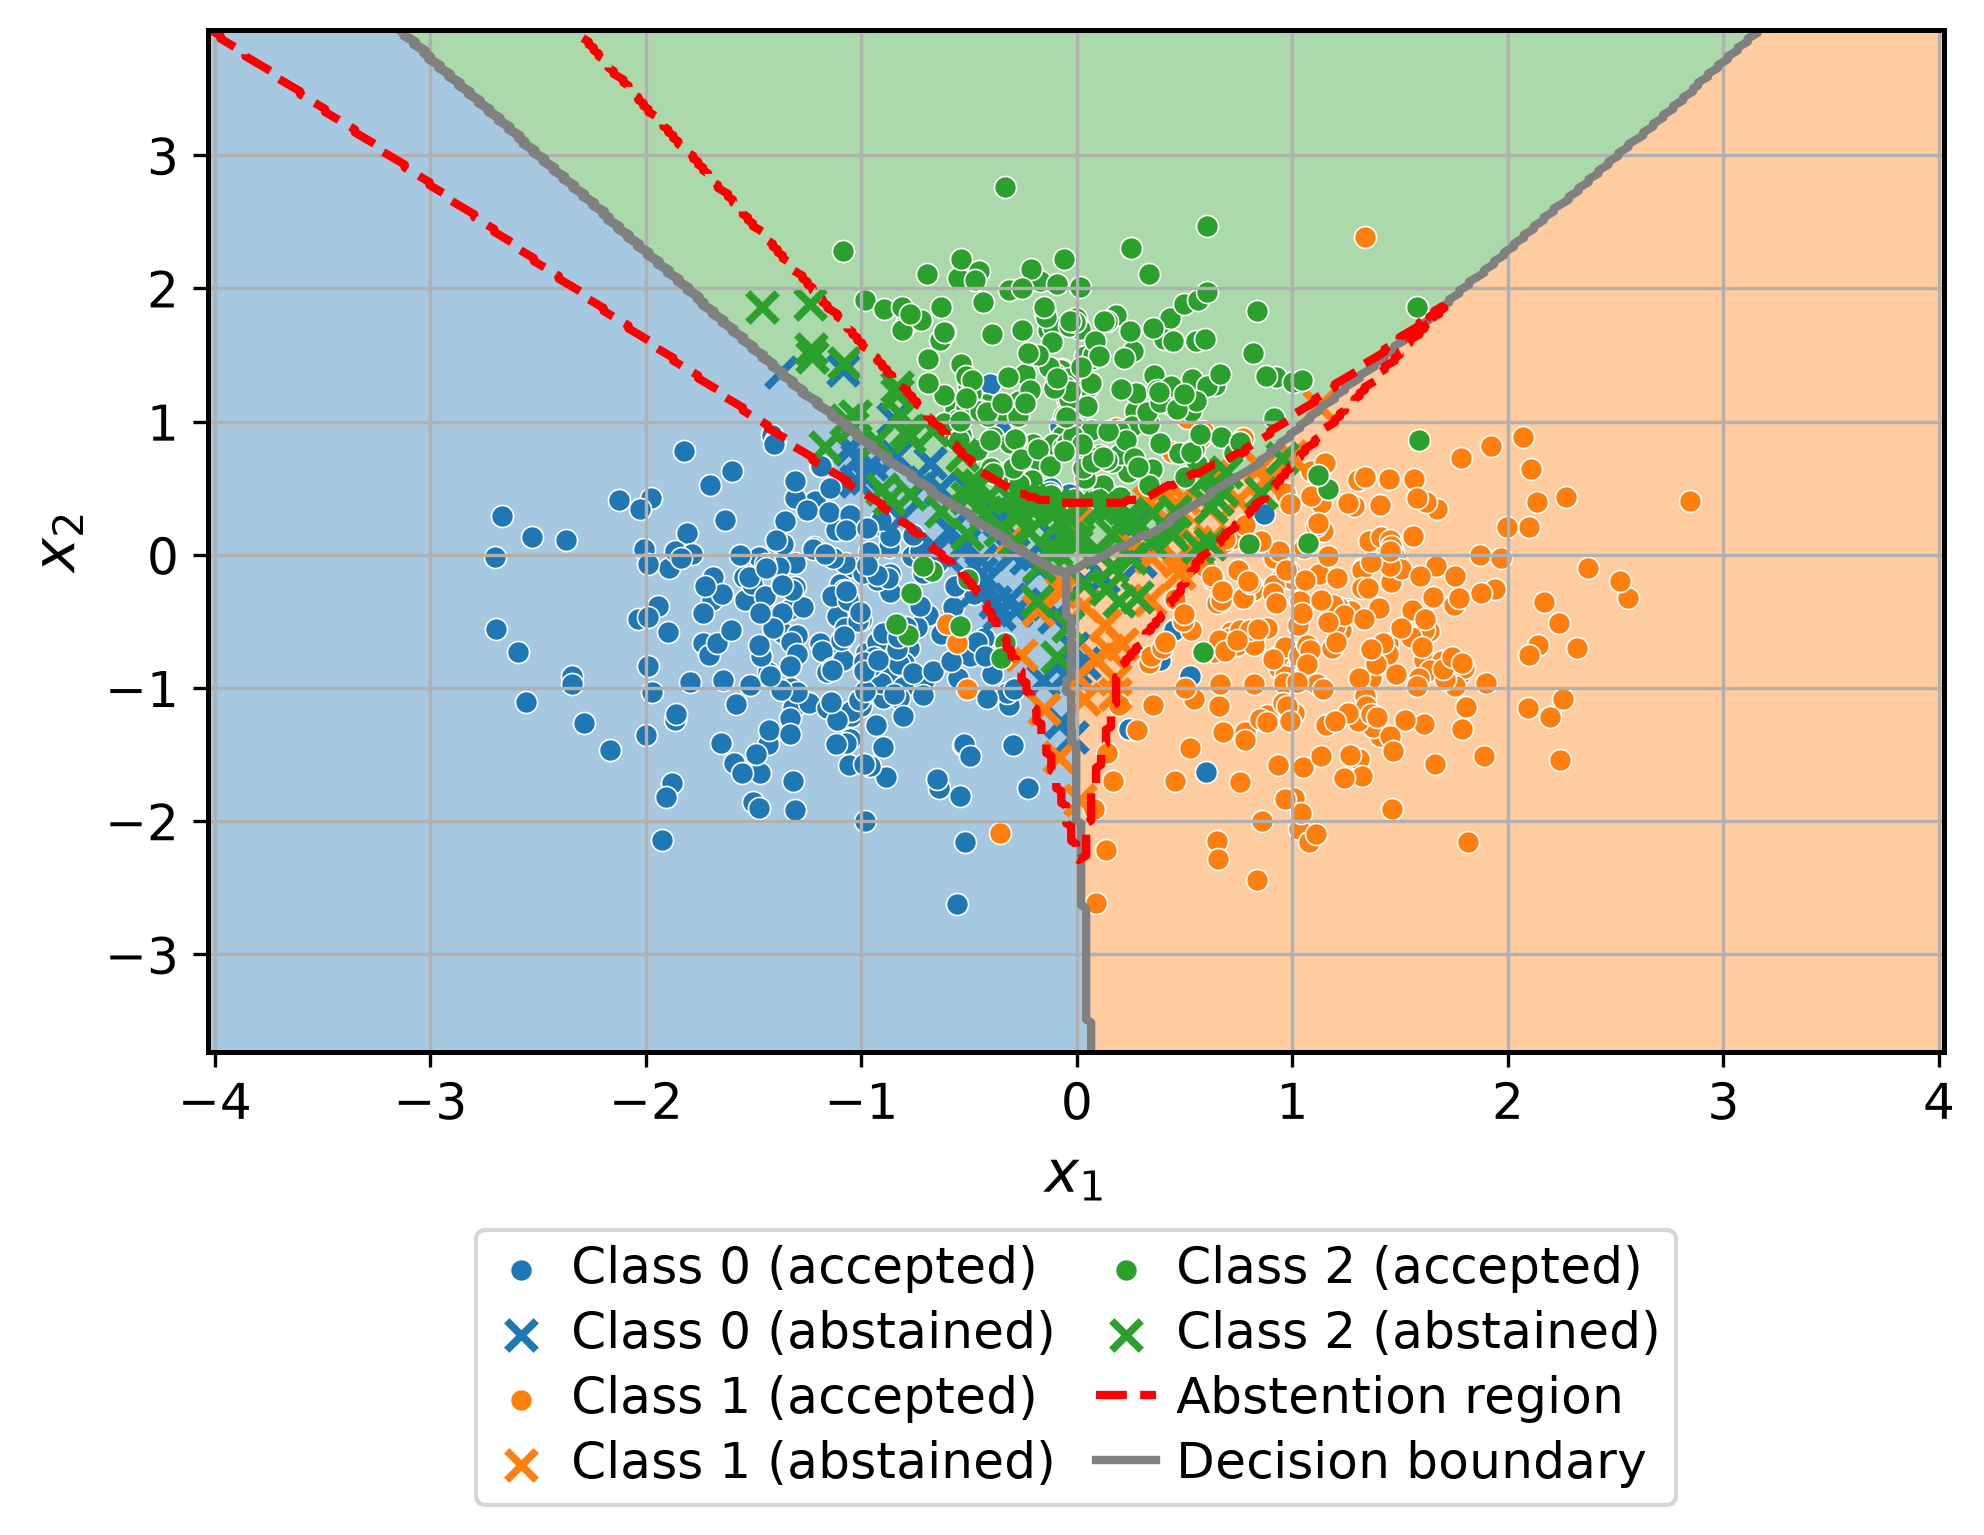
\includegraphics[width=\linewidth]{img/toy_example_rejection_model.png}
        \caption{Decision regions and rejected points.}
        \label{fig:decision_regions}
    \end{subfigure}
    \hspace{0.01\textwidth}
    \begin{minipage}[c]{0.3\textwidth}
        \centering
        \begin{subfigure}{\linewidth}
            \centering
            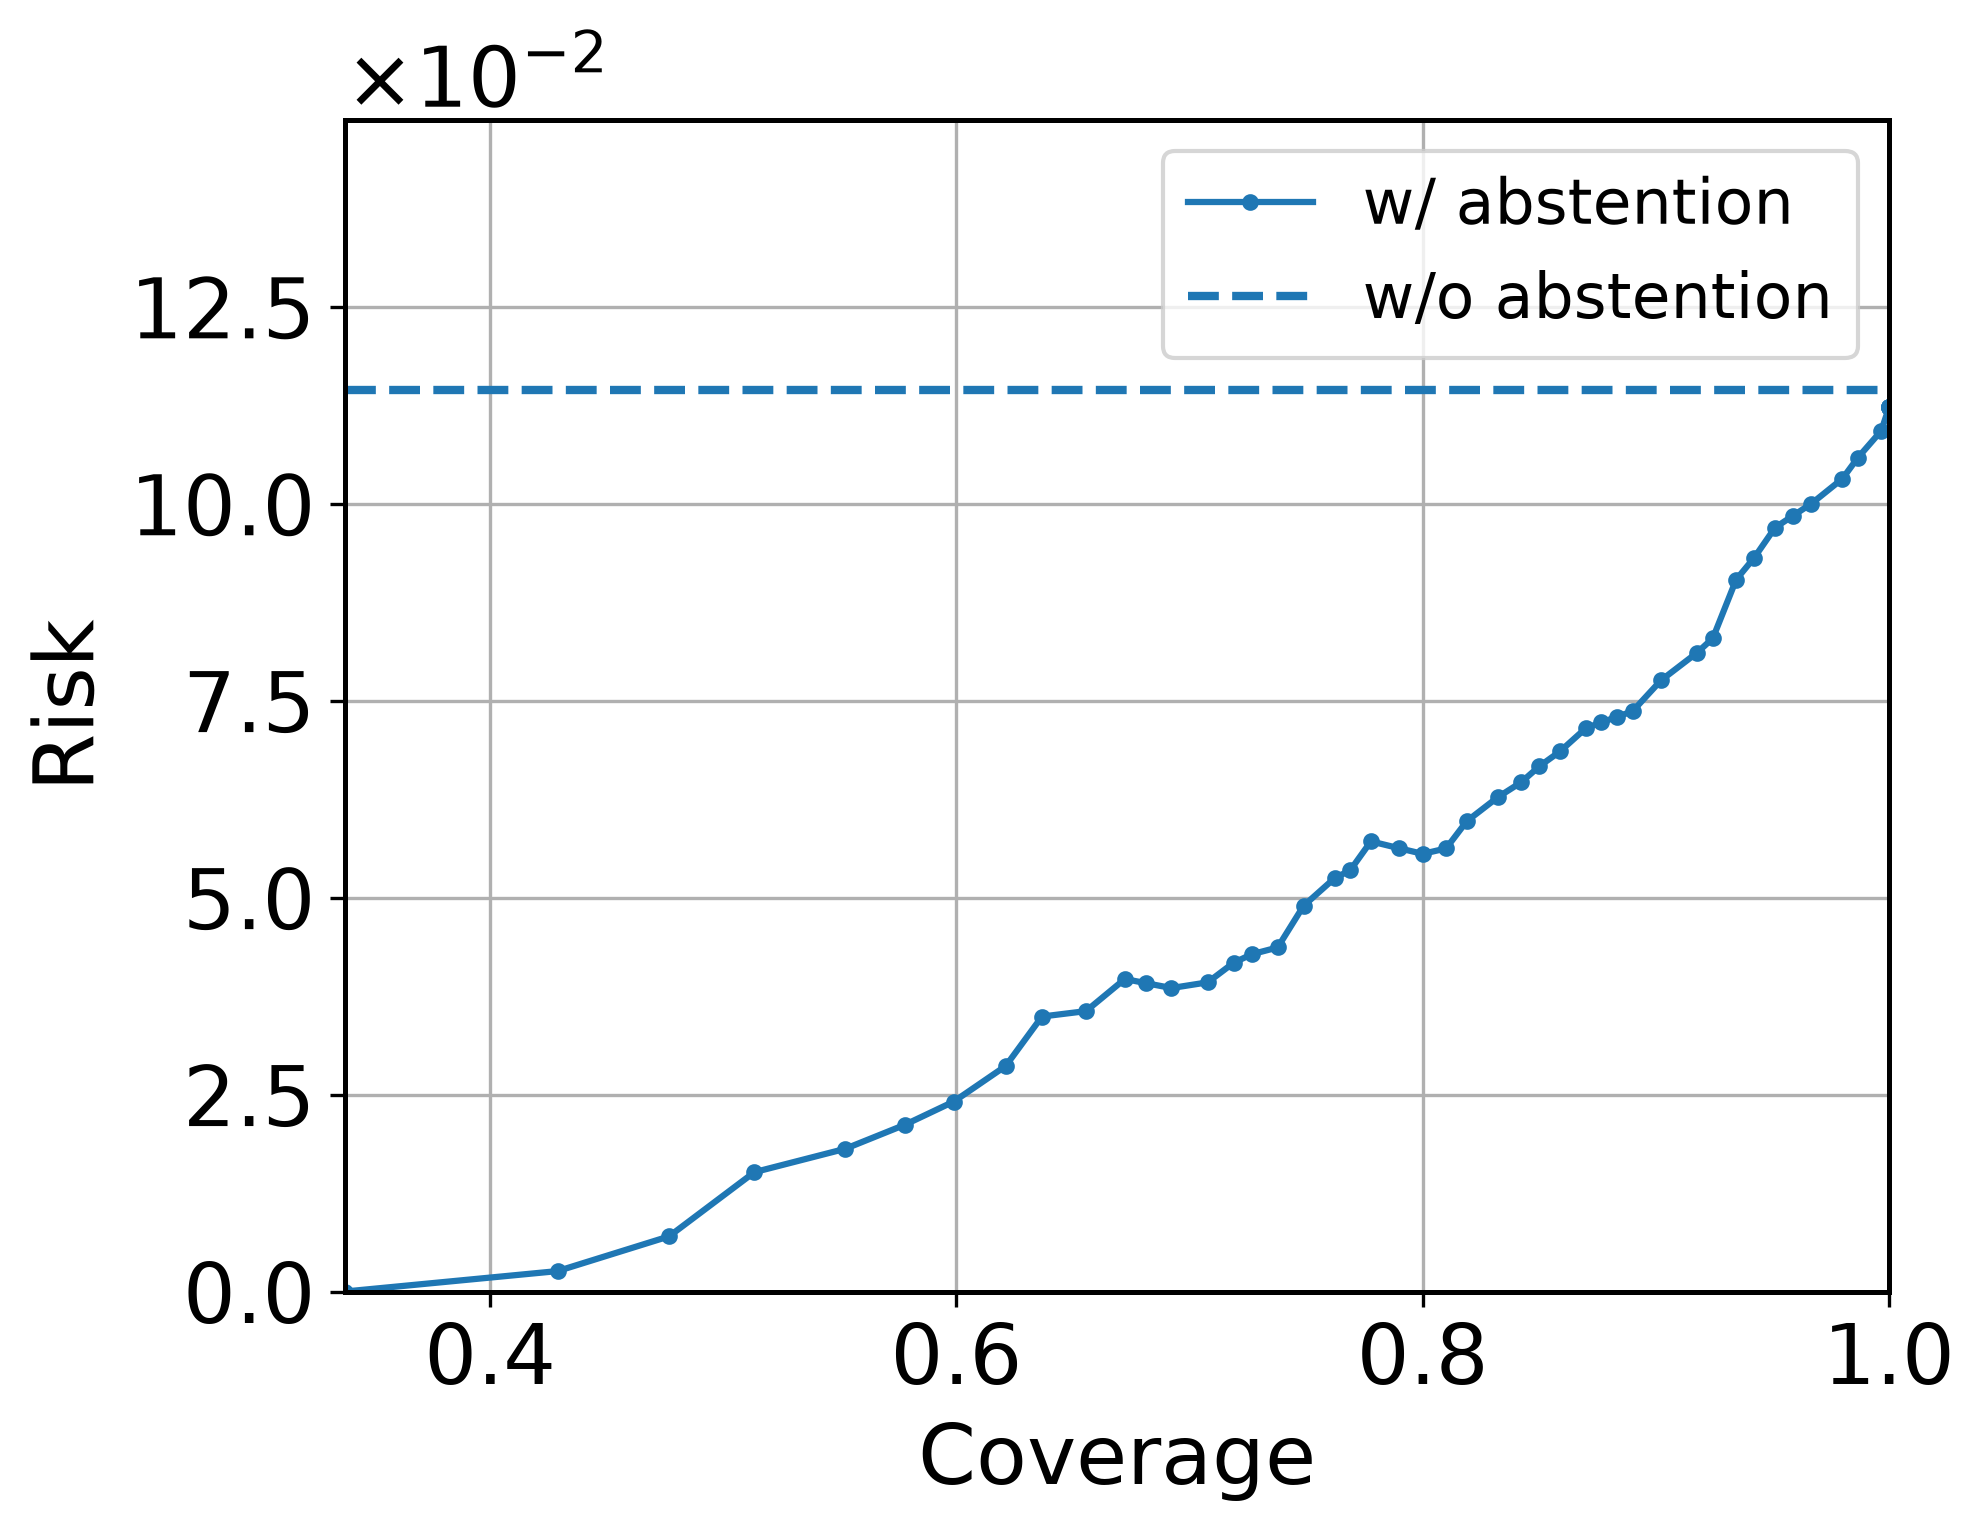
\includegraphics[width=\linewidth]{img/toy_example_selective_risk_curve.png}
            \caption{Selective risk curve.}
            \label{fig:risk_curve}
        \end{subfigure}
        \vspace{0.8em}
        \begin{subfigure}{\linewidth}
            \centering
            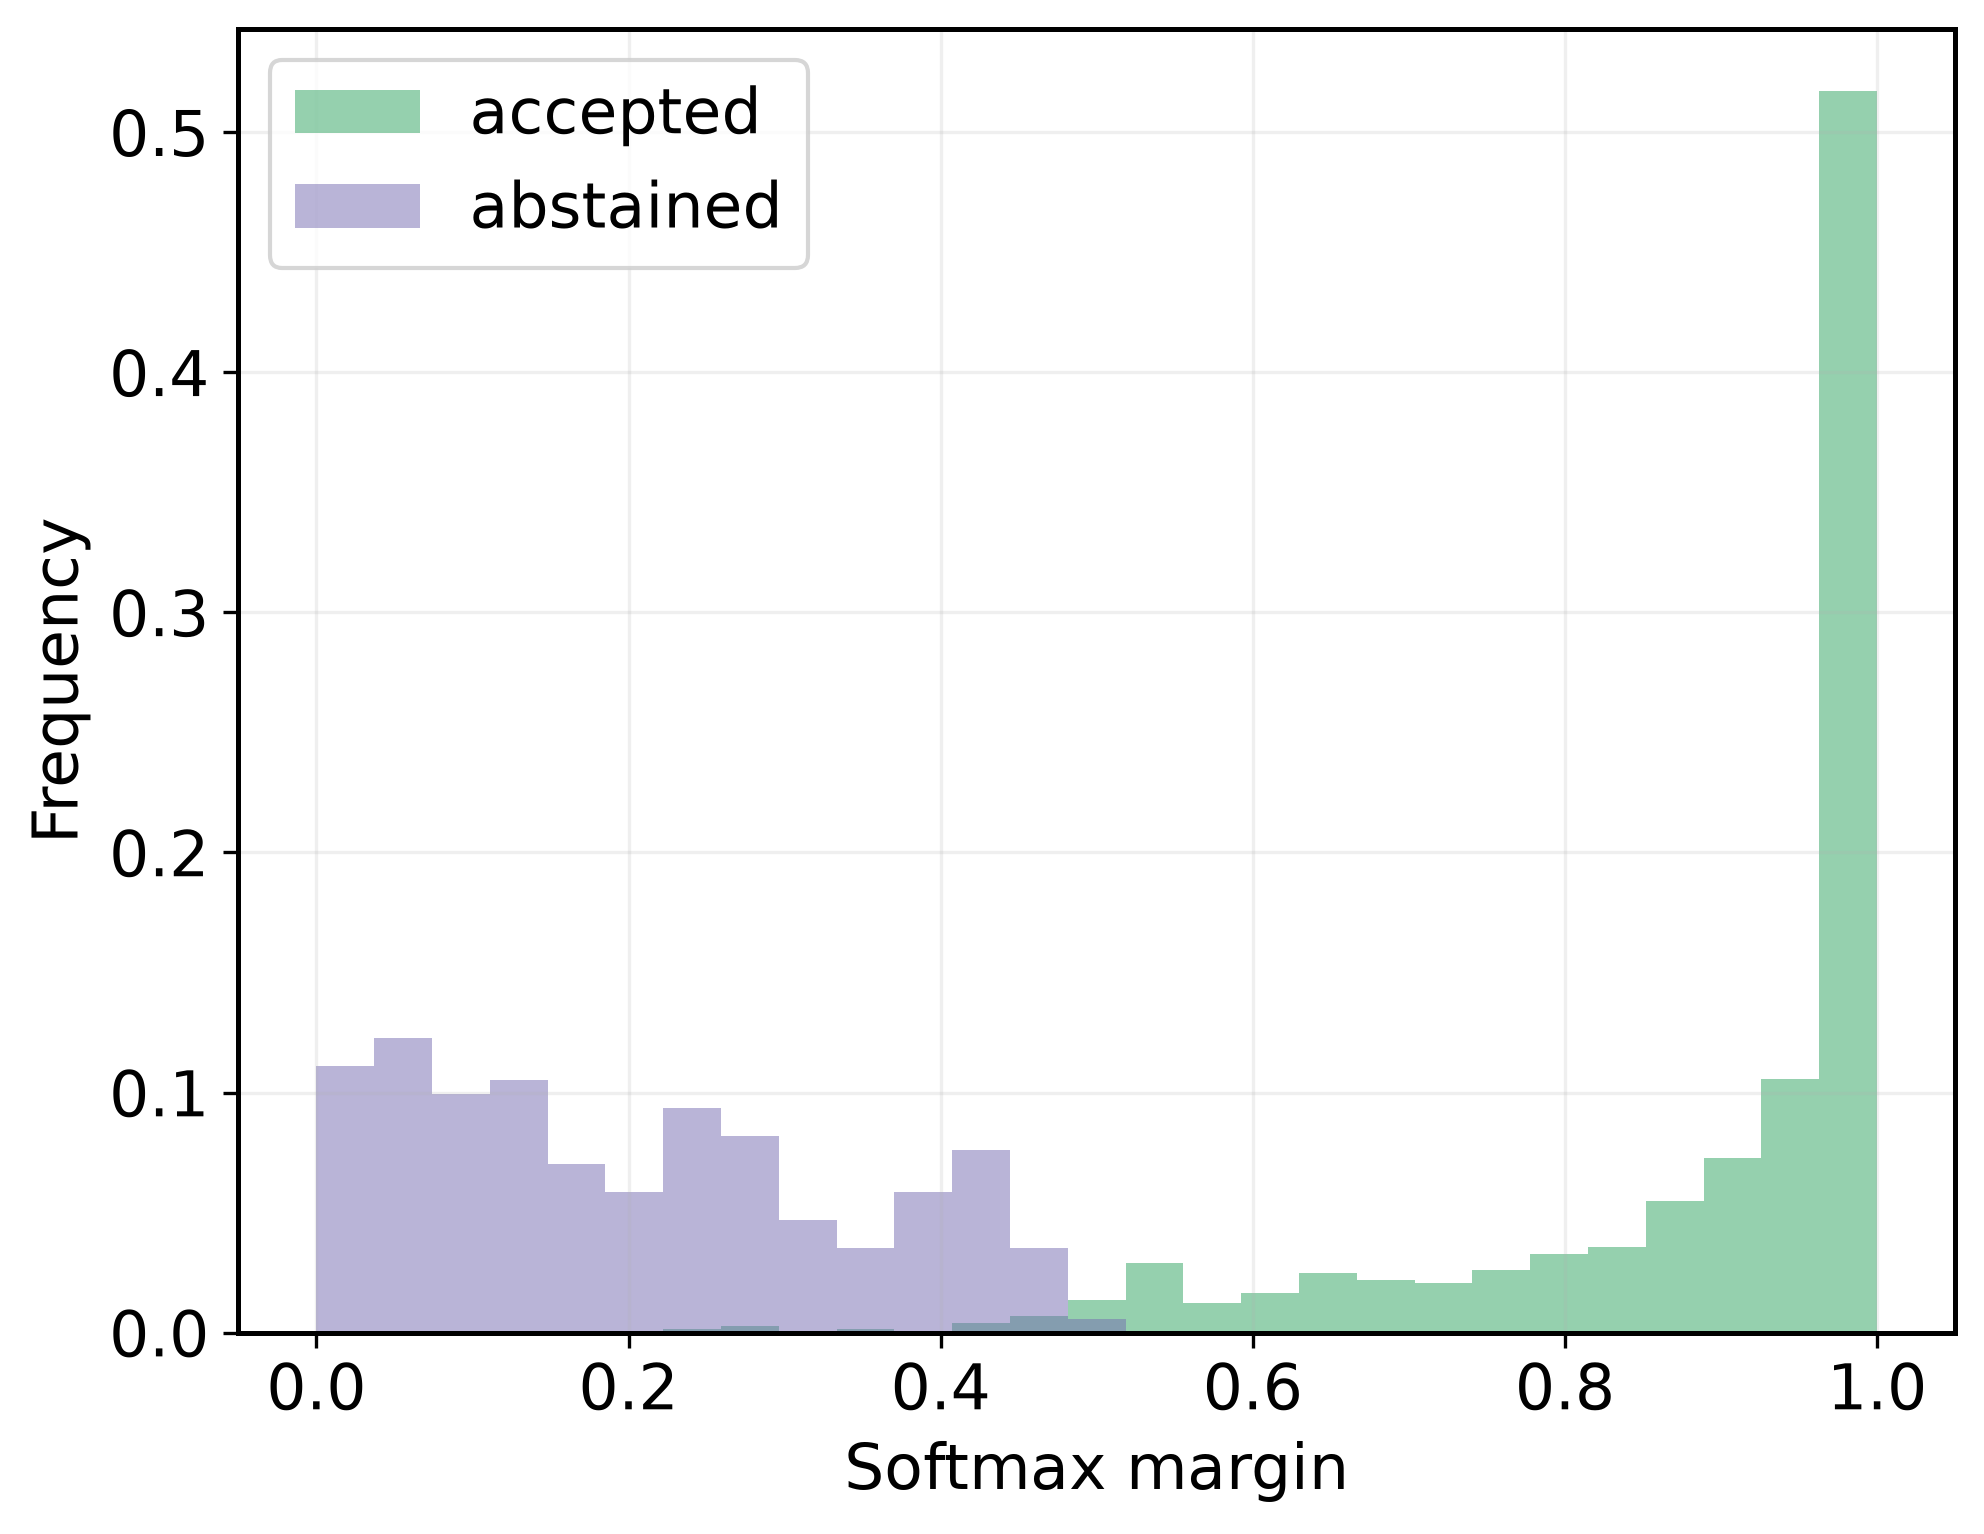
\includegraphics[width=\linewidth]{img/toy_example_margin_histogram.png}
            \caption{Classification margin histogram.}
            \label{fig:margin_histogram}
        \end{subfigure}
    \end{minipage}
    \caption{The impact of abstention on the decision regions, selective risk curve, and classification margin histogram for a toy dataset with bidimensional features and \(C=3\), illustrating how the model can achieve lower classification risk by abstaining on a small fraction of uncertain predictions.}
    \label{fig:illustrative_example}
\end{figure*}